\section{Experimental setup}
\label{sec:setup}

\paragraph{Test images.}
The paper's images (\texttt{galaxy}, \texttt{mri}, \texttt{leopard}, \texttt{elaine})
are not freely redistributable; the paper itself notes that they are standard
images rather than a published dataset. We therefore replaced each one with a
freely available image \emph{of the same kind}, so that every image category the
paper tests is still represented (Fig.~\ref{fig:testimages}):
\begin{itemize}[leftmargin=*,itemsep=1pt]
\item \textbf{satellite} ($256^2$, RestoreTools~\cite{hno}) stands in for
  \texttt{galaxy}: an astronomical image with a black background and thin,
  bright structures. Like the paper's galaxy, it uses $R=3$.
\item \textbf{ct\_head} ($256^2$, a scikit-image CT slice) stands in for
  \texttt{mri}: a medical image with large homogeneous regions and sharp
  anatomical boundaries.
\item \textbf{cat} ($256^2$, scikit-image \texttt{chelsea}) stands in for
  \texttt{leopard}: fur texture, whiskers and eyes.
\item \textbf{portrait} ($512^2$, Kodak \texttt{kodim04}) stands in for
  \texttt{elaine}: a woman in a hat, with smooth skin and sharp contours.
\end{itemize}
For the generalisation study (Sec.~\ref{sec:kodak}), we use 12 further Kodak
images~\cite{kodak}, converted to grayscale and resized to $256^2$
(Fig.~\ref{fig:kodak}), with both blurs at $\delta=10^{-2}$ (24 more problems; we
kept to one noise level to limit the computational cost). All intensities lie in $[0,1]$.

\begin{figure}[t]
\centering
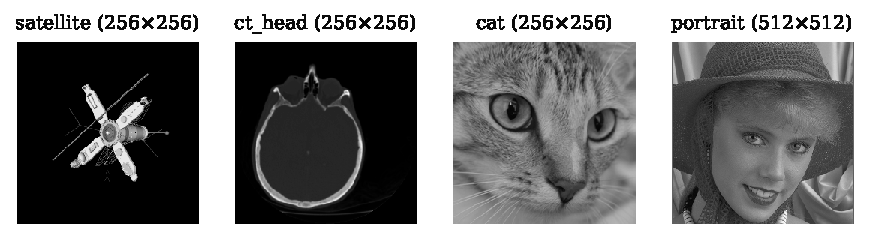
\includegraphics[width=\linewidth]{figures/test_images.pdf}\\[2pt]
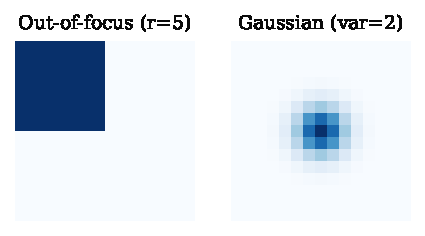
\includegraphics[width=0.48\linewidth]{figures/psfs.pdf}
\caption{Top: the four main test images. Bottom: the two PSFs (central $15\times15$ crop).}
\label{fig:testimages}
\end{figure}

\paragraph{Degradations.}
These follow the paper exactly: (i) a Gaussian PSF with variance 2 (the equivalent
of RestoreTools' \texttt{psfGauss}), and (ii) an out-of-focus disk of radius 5 (the
equivalent of MATLAB's \texttt{fspecial('disk',5)}; boundary pixels are weighted by
their area inside the disk). Both use periodic convolution. Gaussian noise is added
at levels $\delta\in\{2.5\times10^{-2},\,10^{-2},\,5\times10^{-3}\}$, which gives
$4\times2\times3=24$ test problems. The noise seed is fixed per problem, so every
method sees the same $\mathbf b$.

\paragraph{Metrics.}
These are the paper's metrics: relative error
$\mathrm{RE}=\|\hat{\mathbf u}-\mathbf u\|/\|\mathbf u\|$,
$\mathrm{ISNR}=20\log_{10}(\|\mathbf b-\mathbf u\|/\|\hat{\mathbf u}-\mathbf u\|)$ (dB),
and the mean SSIM~\cite{ssim} (Gaussian window, $\sigma=1.5$). We also report PSNR.

\paragraph{Baselines and solvers.}
All methods include the constraint $\mathbf u\ge0$ and use periodic boundaries.
The paper used MATLAB codes (SGP, ADMM, RESPOND), which we do not have, so we
implemented equivalent solvers ourselves:
\begin{itemize}[leftmargin=*,itemsep=1pt]
\item \textbf{TIKH} ($\frac\lambda2\|L\mathbf u\|^2$): solved with the same NP solver.
  Here $H$ is the \emph{exact} Hessian, so NP converges in a few iterations.
\item \textbf{TV}: ADMM~\cite{admm} with splittings $\mathbf z=D\mathbf u$ and $\mathbf w=\mathbf u$; the
  $\mathbf u$-step is an FFT solve, the $\mathbf z$-step an isotropic shrinkage, and the
  $\mathbf w$-step a projection. At most 400 iterations.
\item \textbf{TGV$^2$} ($\alpha_1=\lambda$, $\alpha_0=2\lambda$): the primal--dual hybrid
  gradient method of Chambolle and Pock~\cite{cp}, with the data term dualised so that every
  proximal map is closed-form. We tuned the primal/dual step ratio (30) by checking
  that the objective plateaus; it reaches the minimiser in about 1500 iterations
  (limit 2000).
\end{itemize}

\paragraph{Parameter selection.}
As in the paper, the single parameter of each baseline ($\lambda$ for TIKH, TV
and TGV) and $\epsilon$ for MULTI are chosen to \emph{minimise RE} against the
ground truth. This is an \emph{oracle}, best-case choice for every method. We
implemented it as a coarse log-grid search followed by golden-section refinement,
which expands the bracket automatically if the optimum lies on its edge
(\texttt{experiments/common.py}). MULTI's $\epsilon$ is tuned with a cap of
2000 total NP iterations per run. The reported MULTI run then uses the paper's
full budget (20 outer iterations $\times$ 1000 NP iterations) at the tuned $\epsilon$.
The dense $\epsilon$-sweep of Sec.~\ref{sec:ablation} showed that RE$(\epsilon)$ is not
always unimodal, so a local golden-section search can miss the global optimum. For
every problem we therefore also refine around the best point of the 21-value sweep,
and we keep whichever of the two results is better. This makes the ``oracle'' MULTI
genuinely best-case, like the baselines.
\textbf{MULTI-auto} (Sec.~\ref{sec:auto}) uses no ground truth at all.

\paragraph{MULTI settings.}
These are the paper's values: $\mathrm{Tol}=10^{-1}$ with at most 20 outer
iterations; NP tolerance $10^{-5}$ with at most 1000 iterations;
$R=5$ ($R=3$ for satellite).
